\section{寮食堂と寮生}	\label{sec:cafeteria}\index{りょうしょく@寮食|textbf}
 	熊野寮には、全国の学生寮でも数少ない寮食堂があります。基本的に大学の授業がある平日、朝昼夜の三食が用意され、朝は7時半〜10時、昼は12時〜13時、夜は17時〜17時45分が喫食時間としています。これを見て、「え、そんなに食べる時間短いの? 」と思った方もいるでしょう。ご安心を、そういったご飯の時間内には食べに来られない人のために昼と夜は「残置」\index{りょうしょく@寮食!のざんち@---の残置}というシステムを作ってあり、昼は15時まで、夜は22時までに食べにくるという条件の下で寮食を取り置くことができます! さらに、寮食には利点がいっぱいあります!

  \subsection{寮食は栄養満点! }\index{りょうしょく@寮食!のえいよう@---の栄養}
 	  まず、寮食堂には栄養士の方がいらっしゃり、毎日の栄養計算から献立を作って下さっています。しかもボリュームも満点! しっかり三食食べれば二十歳の成人男性が一日に必要な栄養素を摂取できるのです。朝はパンと乳製品、昼は野菜たっぷりのご飯、夜は主菜を中心とした汁物、副菜二品セット。寮食三食で一日分のビタミン、ミネラルも摂取できるのです。今の若い時分にしっかり栄養を摂っておかないと将来生活習慣病の予備軍になってしまいますが、寮食なら安心ですね。

	\subsection{寮食は安全安心! }
    寮食は安全面にも気を配っています。衛生面はもちろんのこと、使う材料にも気を付けており、肉はほとんど国産、野菜は京野菜をふんだんに使用し、卵は餌から管理されているものを使い、添加物も極力省いています。栄養面でも安全性の面でも身体に良い寮食、これは食べるしかありませんね!

	\subsection{寮食は安い!}\index{りょうしょく@寮食!のねだん@---の値段}
		栄養満点ボリューム満点、おまけに安全安心そんな寮食。でもお高いんでしょう? いえいえ、そんなことはありません! \emphbf{朝は170円、昼は260円、夜は390円と破格! }しかしながらその裏には厨房の栄養士さんや調理員さんの多大なる努力があります。食材を大量購入し、その材料が無駄にならないような調理法、献立を考えた上で栄養も毎日しっかり保つ。さらには夏の冷麺や素麺、冬の鍋物やシチュー、おまけに節分(2月3日)などの季節を感じさせるメニューも登場します。


		\subsection{寮食堂は交流の場}
		食堂と言えばご飯を食べるところ。もちろんそれが食堂の一番の意味ですが、熊野寮食堂は様々な寮生と知り合い交流する場でもあります。熊野寮の食堂は24時間365日開放されています。その管理・運営は寮生と厨房員さんの二人三脚で行われます。なので自分たちの好きな時に自分たちの好きなことができる。これこそまさに自治であり、寮食堂とは自治を象徴する場所なのです! 他愛もない話から昨今の政治の動きなどの難しい話まで、色んな話をしながら寮食を食べるのもあり。時々企画されるコンパやイベント事で朝まで交流するのもあり。炊事当番(食器洗い当番とも言う) では寮生や厨房の方と一緒に働く。自分たちの意志で自由にできる場所です。そしてその意思決定には外部からの干渉は受けません! 友達ができそうになくボッチになりがちな人でも、寮食を食べたりコンパ\index{こんぱ@コンパ}やイベントに参加したりすれば、楽しい出会いが待っていることでしょう。

		ここだけでは熊野寮食堂の素晴らしさは語りつくせません。入寮した暁には、寮食共々是非食堂を利用して有意義な大学生活を送って下さい。



% Please add the following required packages to your document preamble:
% \usepackage{multirow}

\begin{table}[ht]
  {\small
  \caption*{一週間の寮食メニュー(一例)}
  \begin{tabular}{|l|p{9zw}p{9zw}p{9zw}p{9zw}p{9zw}|}
  \hline
   & \multicolumn{1}{l|}{月曜日} & \multicolumn{1}{l|}{火曜日} & \multicolumn{1}{l|}{水曜日} & \multicolumn{1}{l|}{木曜日} & 金曜日 \\ \hline
  \multirow{2}{*}{朝食} & \multicolumn{5}{c|}{パン、牛乳・乳酸飲料・野菜ジュースから一つ選択、チーズ・卵から一つ選択} \\
   & \multicolumn{5}{c|}{*数量限定でカット野菜が用意されており、食パンとチーズと組み合わせピザトーストが作れる} \\ \hline
  \multirow{7}{*}{昼食} & \multicolumn{1}{l|}{そぼろ丼} & \multicolumn{1}{l|}{高菜炒飯} & \multicolumn{1}{l|}{他人丼} & \multicolumn{1}{l|}{オムライス} & 根菜コロッケカレー \\
   & \multicolumn{1}{l|}{味噌汁} & \multicolumn{1}{l|}{サラダ} & \multicolumn{1}{l|}{胡麻和え} & \multicolumn{1}{l|}{サラダ} & ヨーグルトサラダ \\
   & \multicolumn{1}{l|}{} & \multicolumn{1}{l|}{スープ} & \multicolumn{1}{l|}{} & \multicolumn{1}{l|}{スープ} &  \\ \cline{2-6} 
   & \multicolumn{1}{l|}{} & \multicolumn{1}{l|}{スパゲッティ・ミートソース} & \multicolumn{1}{l|}{} & \multicolumn{1}{l|}{豚骨ラーメン} &  \\
   & \multicolumn{1}{l|}{} & \multicolumn{1}{l|}{} & \multicolumn{1}{l|}{} & \multicolumn{1}{l|}{} &  \\
   & \multicolumn{1}{l|}{} & \multicolumn{1}{l|}{} & \multicolumn{1}{l|}{} & \multicolumn{1}{l|}{} &  \\ \cline{2-6} 
   & \multicolumn{5}{c|}{*火曜日と木曜日の昼食は、ご飯と麺の2種類のメニューから選択} \\ \hline
  \multirow{6}{*}{夕食} & \multicolumn{1}{l|}{鰆の柚子かぶら餡かけ} & \multicolumn{1}{l|}{豚肉の照り焼き} & \multicolumn{1}{l|}{赤魚のきのこ餡かけ} & \multicolumn{1}{l|}{プルコギ} & 煮込みハンバーグ \\
   & \multicolumn{1}{l|}{ボイルキャベツ} & \multicolumn{1}{l|}{ボイルキャベツ} & \multicolumn{1}{l|}{ボイルキャベツ} & \multicolumn{1}{l|}{ボイルキャベツ} & ボイルキャベツ \\
   & \multicolumn{1}{l|}{かぼちゃの煮物} & \multicolumn{1}{l|}{ソテー} & \multicolumn{1}{l|}{鶏じゃが} & \multicolumn{1}{l|}{五目煮豆} & オイスター炒め \\
   & \multicolumn{1}{l|}{お浸し} & \multicolumn{1}{l|}{酢の物} & \multicolumn{1}{l|}{お浸し} & \multicolumn{1}{l|}{ゆかり和え} & ピーナツ和え \\
   & \multicolumn{1}{l|}{すまし汁} & \multicolumn{1}{l|}{味噌汁} & \multicolumn{1}{l|}{味噌汁} & \multicolumn{1}{l|}{すまし汁} & 味噌汁 \\ \cline{2-6} 
   & \multicolumn{5}{c|}{*夕食にはご飯がつきます。} \\ \hline
  \end{tabular}
  }
\end{table}
\index{りょうしょく@寮食!めにゅー@---メニュー}


  


寮生が有志でほぼ毎日、寮食のメニューや写真をあげているX(旧twitter)アカウント\index{ついったー@ツイッター!のりょうかんけいあかうんと@---の寮関係アカウント}もあります。興味があればごらんください!

\begin{figure}[h]
  \begin{minipage}[b]{0.5\textwidth}
    \centering
    
\includegraphics[width=3cm]{gazo/QR_ryoshoku_bot.png}
    \subcaption{\url{https://twitter.com/ryosyoku_buono}
    \\熊野寮寮食bot Twitter(\url{@ryosyoku_buono})}
  \end{minipage}
  \begin{minipage}[b]{0.5\textwidth}
    \centering
    
\includegraphics[width=3cm]{gazo/QR_ajiri.png}
    \subcaption{\url{https://bit.ly/3rL87Vk}\\ 熊野あじり Twitter\url{@kumano_ajiri}}
  \end{minipage}
\end{figure}


\begin{figure}[H]
  \centering
  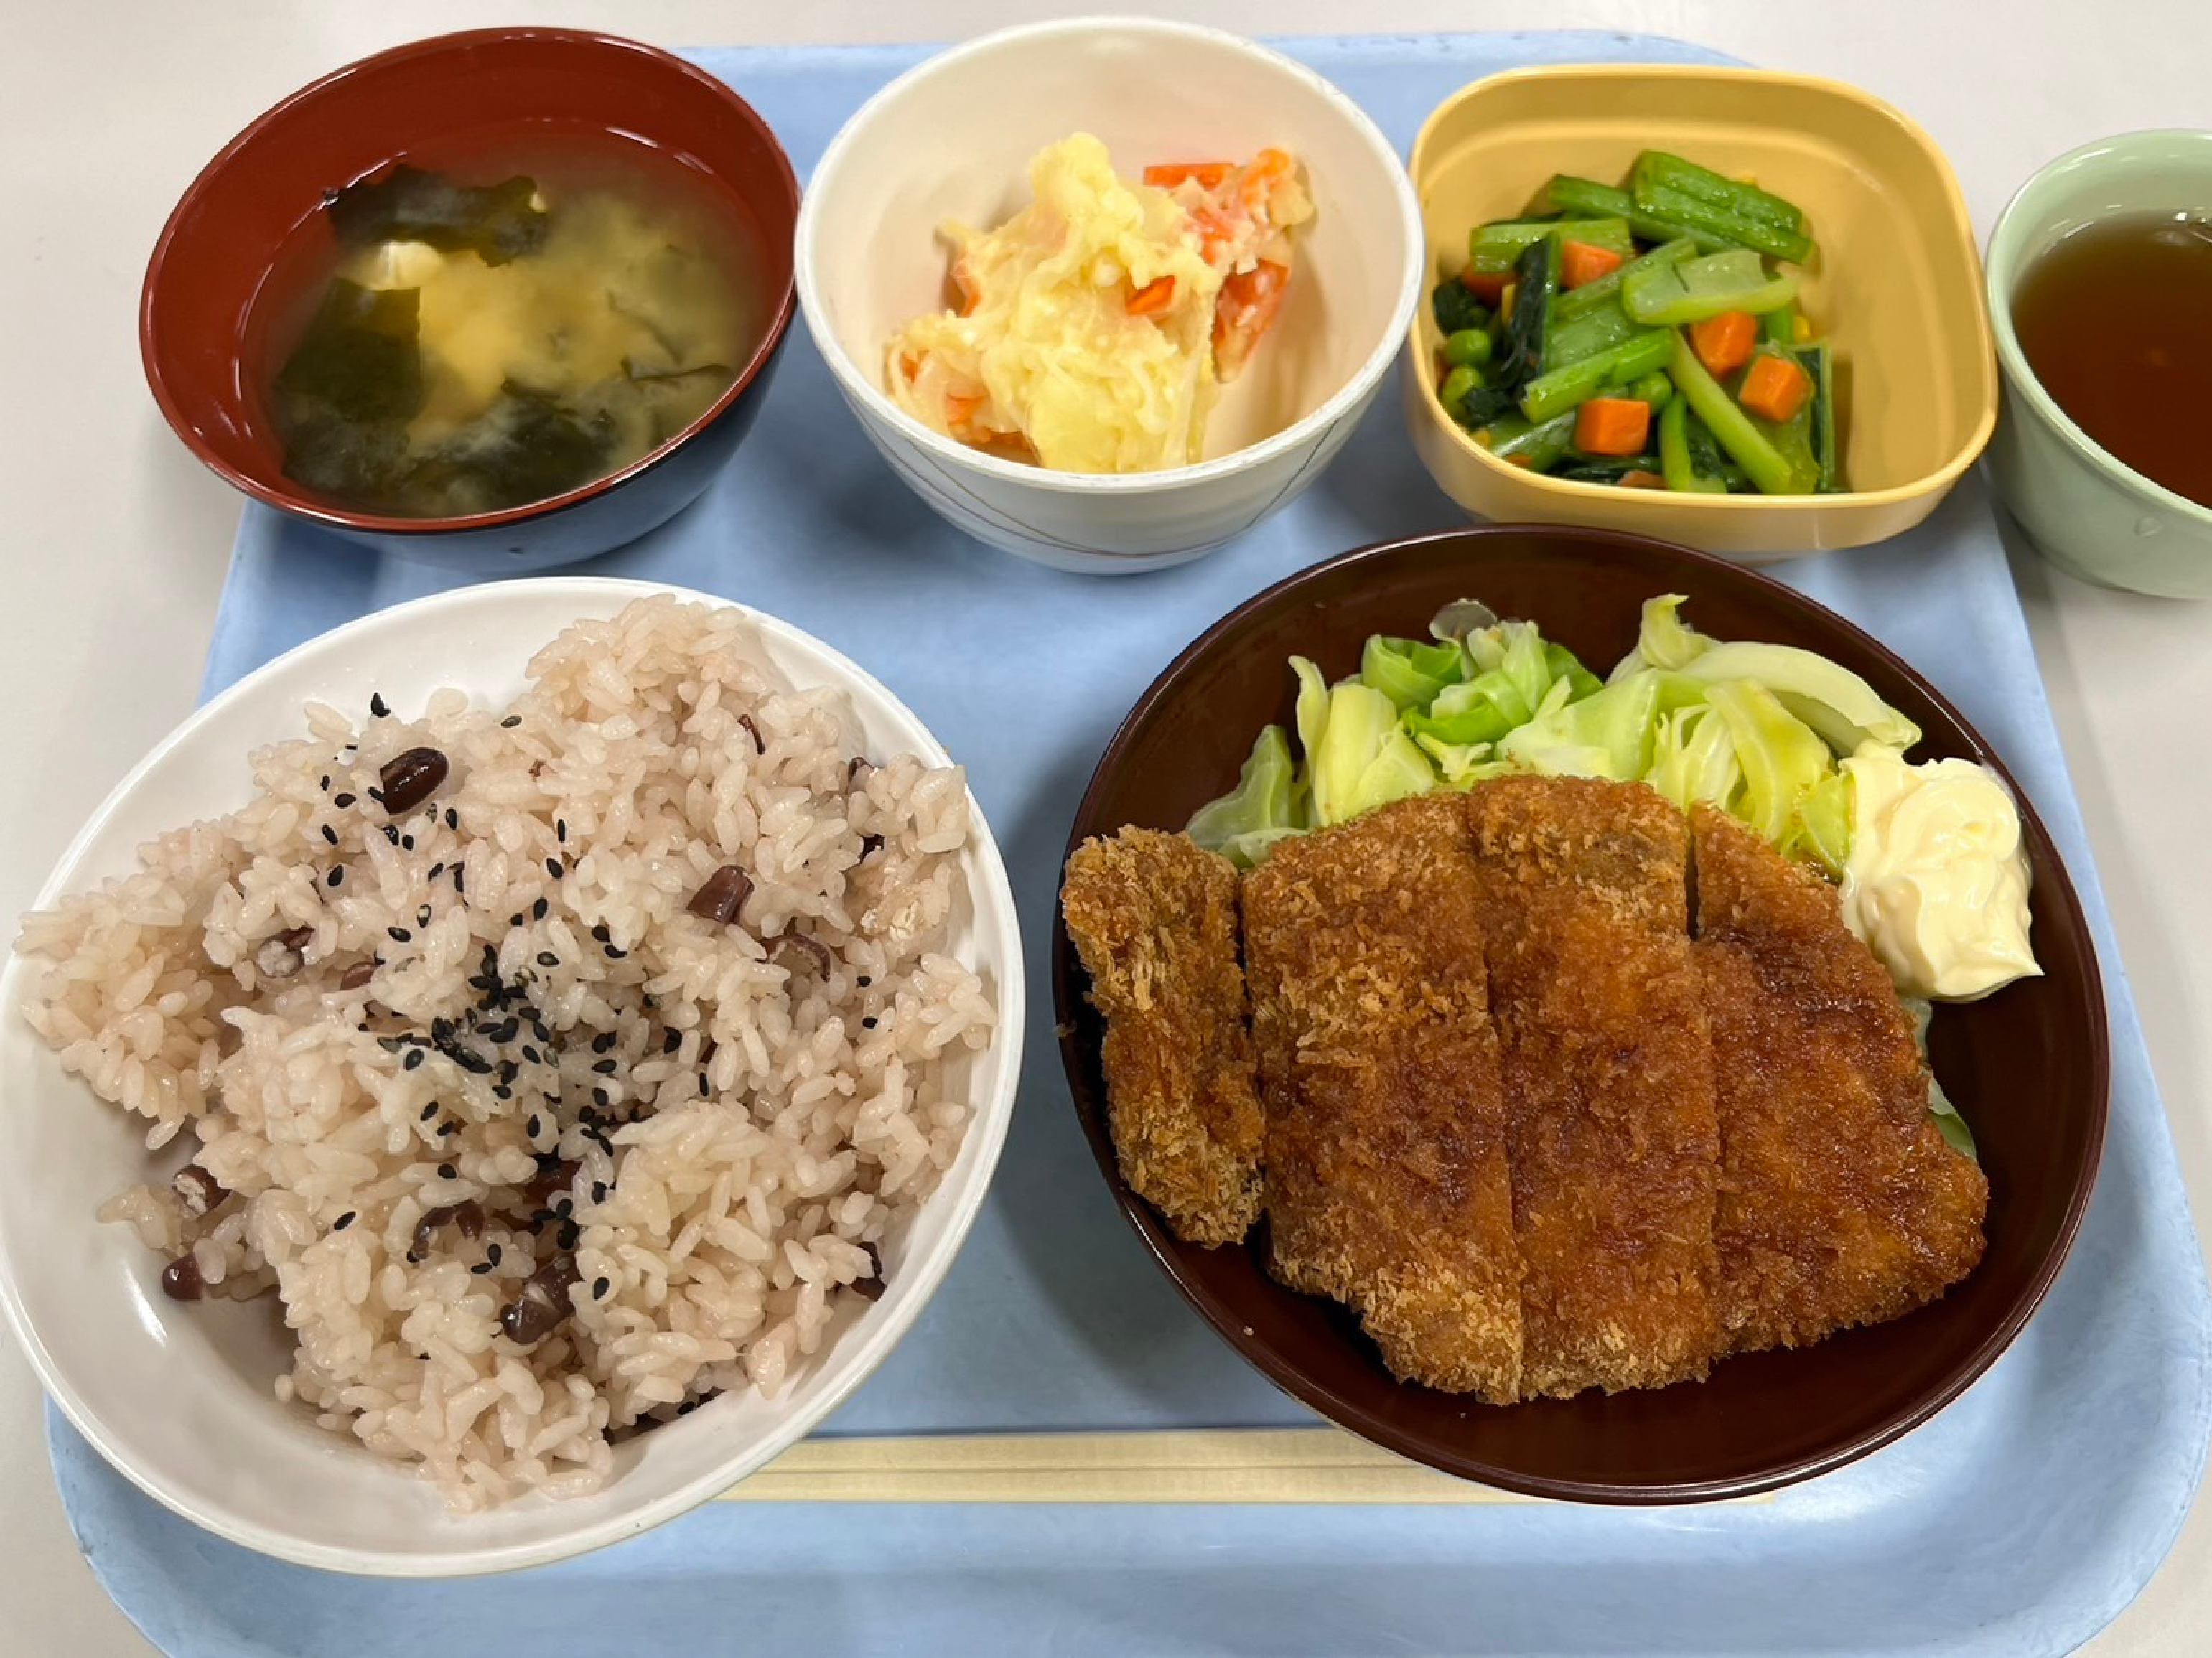
\includegraphics[width=5cm]{gazo/sekihan.pdf}
  \subcaption{{\small この日の夕食は赤飯に豚カツの豪華メニュー}}
\end{figure}